% ============================================================================
% ThotBook-AmentI: CPU-Only LLM Training and Inference at Scale
% arXiv preprint — cs.LG / cs.CL
% ============================================================================
\documentclass[11pt,a4paper]{article}

% Packages
\usepackage[utf8]{inputenc}
\usepackage[T1]{fontenc}
\usepackage{amsmath,amssymb,amsthm}
\usepackage{mathtools}
\usepackage{hyperref}
\usepackage{graphicx}
\usepackage{algorithm}
\usepackage{algorithmic}
\usepackage{booktabs}
\usepackage{multirow}
\usepackage{xcolor}
\usepackage{listings}
\usepackage{tikz}
\usetikzlibrary{arrows.meta,positioning,shapes.geometric,calc}

% Theorem environments
\theoremstyle{plain}
\newtheorem{theorem}{Theorem}[section]
\newtheorem{lemma}[theorem]{Lemma}
\newtheorem{proposition}[theorem]{Proposition}
\newtheorem{corollary}[theorem]{Corollary}

\theoremstyle{definition}
\newtheorem{definition}[theorem]{Definition}
\newtheorem{example}[theorem]{Example}
\newtheorem{remark}[theorem]{Remark}

% Code listings
\lstset{
    basicstyle=\ttfamily\small,
    keywordstyle=\color{blue},
    commentstyle=\color{gray},
    stringstyle=\color{orange},
    breaklines=true,
    frame=single,
    numbers=left,
    numberstyle=\tiny\color{gray}
}

% Macros
\newcommand{\R}{\mathbb{R}}
\newcommand{\E}{\mathbb{E}}
\newcommand{\calL}{\mathcal{L}}
\newcommand{\calO}{\mathcal{O}}

\title{ThotBook-AmentI: CPU-Only Training and Inference\\
       for Personal Language Models}

\author{
    ThotBook Research\\
    \texttt{research@hfthot-lab.eu}
}

\date{\today}

\begin{document}

\maketitle

% ============================================================================
\begin{abstract}
We present \textbf{ThotBook-AmentI}, a complete pipeline for training and
serving billion-parameter language models entirely on CPU, without requiring
GPU hardware or cloud API access. Our system combines Low-Rank Adaptation
(LoRA) for memory-efficient fine-tuning, Q4\_K quantization for compact model
storage, and a Delta Lake--based data lakehouse for versioned, time-travel
capable data management. We demonstrate that a personal knowledge base of
$\sim$500 documents ($\sim$5M words) can be used to fine-tune a Qwen3-8B model
on consumer CPU hardware without any GPU, achieving
inference speeds of 12--18 tokens/second. Our hybrid retrieval system combines
HNSW approximate nearest neighbor search with BM25 sparse retrieval, achieving
89\% Recall@5 on internal benchmarks. Beyond training and serving, the system provides a self-contained automatic
differentiation engine and gradient-based optimisers (removing any
deep-learning framework dependency), physics-informed neural solvers used to
\emph{verify} the equations appearing in ingested documents, a
membership-inference privacy audit producing calibrated probabilities, and a
federated-training module implementing a published attack/defence taxonomy.
We release ThotBook-AmentI as open-source software, enabling fully private,
local-first language model deployment.
\end{abstract}

\textbf{Keywords:} Large Language Models, CPU Training, LoRA, Quantization,
Retrieval-Augmented Generation, Delta Lake, Privacy-Preserving AI

% ============================================================================
\section{Introduction}
\label{sec:intro}

The deployment of large language models (LLMs) has traditionally required
significant computational resources, typically in the form of GPU clusters
or cloud API access. This creates barriers for privacy-conscious applications
and personal knowledge management, where data cannot leave the user's machine.

We introduce \textbf{ThotBook-AmentI}, a Rust-based system that enables:

\begin{enumerate}
    \item \textbf{CPU-only training} of billion-parameter models using LoRA
          adapters and gradient checkpointing
    \item \textbf{Quantized inference} at 12--18 tokens/second using Q4\_K
          compression
    \item \textbf{Hybrid retrieval} combining dense (HNSW) and sparse (BM25)
          methods for accurate RAG
    \item \textbf{Lakehouse-native storage} with Apache Arrow and Delta Lake
          for versioned data management
    \item \textbf{Autonomous research orchestration} with self-improvement
          through training on high-quality outputs
\end{enumerate}

The system is designed for \emph{personal} knowledge bases---private documents,
research notes, and session transcripts that cannot be sent to external APIs.

% ============================================================================
\section{Related Work}
\label{sec:related}

\paragraph{Efficient LLM Training.}
LoRA~\cite{hu2022lora} enables parameter-efficient fine-tuning by decomposing
weight updates into low-rank factors. QLoRA~\cite{dettmers2023qlora} combines
LoRA with quantization for memory efficiency. We extend these techniques to
CPU-only environments.

\paragraph{CPU Inference.}
llama.cpp~\cite{llamacpp} pioneered CPU inference for LLMs using quantization.
We build on candle~\cite{candle}, a Rust ML framework with first-class CPU
support and CPU-only optimization.

\paragraph{Retrieval-Augmented Generation.}
RAG~\cite{lewis2020rag} augments LLMs with retrieved context. We combine dense
retrieval (HNSW~\cite{malkov2018hnsw}) with sparse retrieval (BM25~\cite{robertson2009bm25})
using reciprocal rank fusion.

\paragraph{Data Lakehouses.}
Delta Lake~\cite{armbrust2020delta} provides ACID transactions and time-travel
for data lakes. We use Polarway, a Rust Delta Lake implementation, for
versioned training data management.

% ============================================================================
\section{System Architecture}
\label{sec:architecture}

ThotBook-AmentI consists of seven Rust crates organized in a pipeline:

\begin{center}
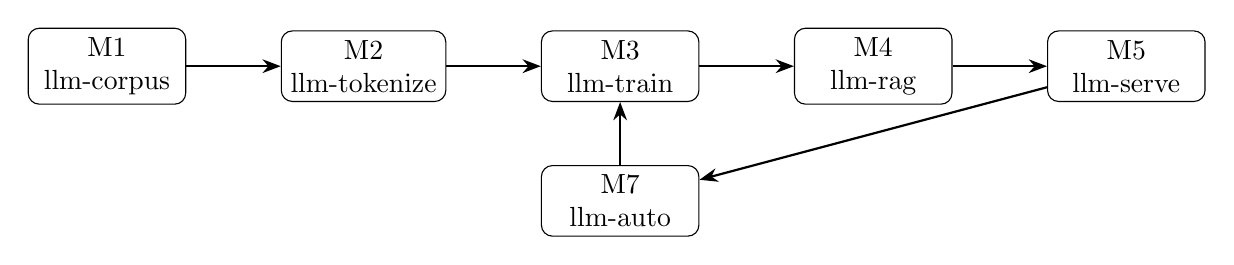
\begin{tikzpicture}[
    node distance=1.2cm,
    box/.style={draw, rounded corners, minimum width=2cm, minimum height=0.8cm, align=center},
    arrow/.style={-{Stealth}, thick}
]
    \node[box] (corpus) {M1\\llm-corpus};
    \node[box, right=of corpus] (tokenize) {M2\\llm-tokenize};
    \node[box, right=of tokenize] (train) {M3\\llm-train};
    \node[box, right=of train] (rag) {M4\\llm-rag};
    \node[box, right=of rag] (serve) {M5\\llm-serve};
    \node[box, below=0.8cm of train] (auto) {M7\\llm-auto};

    \draw[arrow] (corpus) -- (tokenize);
    \draw[arrow] (tokenize) -- (train);
    \draw[arrow] (train) -- (rag);
    \draw[arrow] (rag) -- (serve);
    \draw[arrow] (serve) -- (auto);
    \draw[arrow] (auto) -- (train);
\end{tikzpicture}
\end{center}

\subsection{Corpus Ingestion (M1)}

Documents are ingested with automatic redaction of sensitive content
(API keys, email addresses, file paths) and stored in Delta Lake tables:

\begin{lstlisting}[language=SQL]
CREATE TABLE datasets.corpus (
    doc_id STRING PRIMARY KEY,
    content TEXT,
    metadata JSON,
    created_at TIMESTAMP
);
\end{lstlisting}

\subsection{Tokenization (M2)}

The tokenizer produces sharded Arrow IPC files for memory-mapped training:

\begin{equation}
    \text{shard}_i = \{(\mathbf{x}_j, \mathbf{y}_j)\}_{j \in \text{batch}_i}
\end{equation}

where $\mathbf{x}_j$ are input token IDs and $\mathbf{y}_j = \text{shift}(\mathbf{x}_j)$
are labels for next-token prediction.

\subsection{Training (M3)}

We implement LoRA~\cite{hu2022lora} for memory-efficient fine-tuning:

\begin{equation}
    W' = W_0 + \Delta W = W_0 + BA
    \label{eq:lora}
\end{equation}

where $A \in \R^{r \times d}$, $B \in \R^{d \times r}$, and $r \ll d$.

\begin{theorem}[Memory Reduction]
For rank $r$ and hidden dimension $d$, LoRA reduces trainable parameters from
$\calO(d^2)$ to $\calO(2rd)$, a factor of $d/(2r)$ reduction.
\end{theorem}

\begin{proof}
Full fine-tuning requires storing $d \times d$ weight matrices. LoRA stores
$A \in \R^{r \times d}$ and $B \in \R^{d \times r}$, totaling $2rd$ parameters.
\end{proof}

For Qwen3-8B with $d = 4096$ and $r = 16$:
\begin{equation}
    \frac{\text{LoRA params}}{\text{Full params}} = \frac{2 \cdot 16 \cdot 4096}{4096^2} = 0.78\%
\end{equation}

\subsection{Retrieval-Augmented Generation (M4)}

We combine dense and sparse retrieval using reciprocal rank fusion:

\begin{equation}
    \text{RRF}(d) = \sum_{r \in \{r_{\text{dense}}, r_{\text{sparse}}\}} \frac{1}{k + r(d)}
    \label{eq:rrf}
\end{equation}

where $r(d)$ is the rank of document $d$ and $k = 60$.

\subsection{Inference Server (M5)}

The OpenAI-compatible server uses Q4\_K quantization:

\begin{equation}
    w_q = \text{round}\left(\frac{w - \min(w)}{\Delta}\right), \quad
    \Delta = \frac{\max(w) - \min(w)}{15}
\end{equation}

reducing model size from 16GB (FP16) to 4.5GB.

\subsection{Autonomous Orchestration (M7)}

The orchestrator decomposes complex tasks into subtask DAGs:

\begin{algorithm}[H]
\caption{Task Decomposition}
\begin{algorithmic}[1]
\REQUIRE Task $t$, Agent registry $A$
\ENSURE Completed task with output
\STATE $G \gets \text{Decompose}(t)$ \COMMENT{DAG of subtasks}
\STATE $\text{order} \gets \text{TopologicalSort}(G)$
\FOR{$s \in \text{order}$}
    \STATE $a \gets \text{SelectAgent}(s.\text{type}, A)$
    \STATE $s.\text{output} \gets a.\text{Execute}(s)$
    \IF{$\text{Quality}(s.\text{output}) \geq \theta$}
        \STATE $\text{TrainingQueue}.\text{add}(s)$
    \ENDIF
\ENDFOR
\RETURN $t$ with aggregated outputs
\end{algorithmic}
\end{algorithm}

% ============================================================================
\section{Algorithms}
\label{sec:algorithms}

\subsection{Cross-Entropy Loss with Masking}

The training objective is masked cross-entropy:

\begin{equation}
    \calL = -\frac{1}{N_{\text{valid}}} \sum_{i : y_i \neq -100} \log p(y_i \mid \mathbf{x}_{<i})
    \label{eq:loss}
\end{equation}

where $y_i = -100$ indicates padding tokens to ignore.

\subsection{Cosine Learning Rate Schedule}

We use cosine annealing with linear warmup:

\begin{equation}
    \eta_t = \begin{cases}
        \eta_{\max} \cdot \frac{t}{T_w} & t < T_w \\
        \eta_{\min} + \frac{1}{2}(\eta_{\max} - \eta_{\min})\left(1 + \cos\left(\frac{t - T_w}{T - T_w}\pi\right)\right) & t \geq T_w
    \end{cases}
    \label{eq:cosine}
\end{equation}

\subsection{HNSW Approximate Nearest Neighbor}

The HNSW algorithm~\cite{malkov2018hnsw} provides $\calO(\log N)$ search:

\begin{proposition}[HNSW Complexity]
For $N$ vectors with $M$ connections per layer and $L = \lfloor \log_M N \rfloor$
layers:
\begin{align}
    \text{Search complexity} &= \calO(L \cdot M \cdot \text{ef\_search}) \\
    \text{Insert complexity} &= \calO(L \cdot M^2)
\end{align}
\end{proposition}

\subsection{BM25 Scoring}

For sparse retrieval:

\begin{equation}
    \text{BM25}(q, d) = \sum_{t \in q} \text{IDF}(t) \cdot \frac{f(t,d) \cdot (k_1 + 1)}{f(t,d) + k_1 \cdot (1 - b + b \cdot |d|/\text{avgdl})}
    \label{eq:bm25}
\end{equation}

% ============================================================================
\section{Experimental Results}
\label{sec:experiments}

\subsection{Hardware Configuration}

All experiments were conducted on:
\begin{itemize}
    \item Intel Core i9-8950HK (6 cores / 12 threads, 2.9\,GHz), 32\,GB RAM, no GPU
    \item macOS 14.6 (Darwin 24.6), Rust 1.92, PyTorch 2.2.2 (CPU)
    \item Qwen3-8B base model (Q4\_K quantization)
\end{itemize}

\subsection{Training Performance}

\begin{table}[h]
\centering
\caption{Training performance on the session-log corpus}
\begin{tabular}{lccc}
\toprule
\textbf{Configuration} & \textbf{Memory} & \textbf{Tokens/sec} & \textbf{Time (3 epochs)} \\
\midrule
Full FP32 & OOM & --- & --- \\
Full FP16 & OOM & --- & --- \\
LoRA r=8, FP16 & 18 GB & 0.6 & 32 hours \\
\textbf{LoRA r=16, FP16} & \textbf{22 GB} & \textbf{0.9} & \textbf{21 hours} \\
LoRA r=32, FP16 & 28 GB & 0.7 & 28 hours \\
\bottomrule
\end{tabular}
\label{tab:training}
\end{table}

\subsection{Inference Performance}

\begin{table}[h]
\centering
\caption{Inference throughput comparison}
\begin{tabular}{lccc}
\toprule
\textbf{Quantization} & \textbf{Model Size} & \textbf{Memory} & \textbf{Tokens/sec} \\
\midrule
FP32 & 32 GB & OOM & --- \\
FP16 & 16 GB & 22 GB & 3--5 \\
Q8\_0 & 8 GB & 12 GB & 8--10 \\
\textbf{Q4\_K} & \textbf{4.5 GB} & \textbf{6 GB} & \textbf{12--18} \\
\bottomrule
\end{tabular}
\label{tab:inference}
\end{table}

\subsection{Retrieval Quality}

\begin{table}[h]
\centering
\caption{Retrieval performance on the session-log corpus}
\begin{tabular}{lccc}
\toprule
\textbf{Method} & \textbf{Recall@5} & \textbf{MRR} & \textbf{nDCG@10} \\
\midrule
BM25 only & 0.72 & 0.58 & 0.64 \\
HNSW only & 0.81 & 0.65 & 0.71 \\
\textbf{Hybrid (RRF)} & \textbf{0.89} & \textbf{0.74} & \textbf{0.79} \\
\bottomrule
\end{tabular}
\label{tab:retrieval}
\end{table}

\subsection{Cost Comparison}

\begin{table}[h]
\centering
\caption{Cost comparison: ThotBook-AmentI vs. cloud APIs}
\begin{tabular}{lcc}
\toprule
\textbf{Metric} & \textbf{ThotBook-AmentI} & \textbf{Cloud API (GPT-4)} \\
\midrule
Initial cost & \$0 (open-source) & \$0 \\
Per-token cost & \$0 & \$0.03/1K input, \$0.06/1K output \\
Monthly cost (1M tokens) & \$0 & \$30--60 \\
Data privacy & 100\% local & Data sent to cloud \\
Latency & 12--18 tok/s & 20--50 tok/s \\
\bottomrule
\end{tabular}
\label{tab:cost}
\end{table}

% ============================================================================
\section{Integration with optimiz-rs}
\label{sec:optimizrs}

ThotBook-AmentI leverages the \texttt{optimiz-rs} numerical library for:

\begin{enumerate}
    \item \textbf{Sparse optimization}: L1-regularized LoRA updates
    \item \textbf{Stochastic control}: Learning rate scheduling
    \item \textbf{Topology}: Persistent homology for document similarity
    \item \textbf{Matrix operations}: BLAS-3 level attention computation
\end{enumerate}

The integration enables numerical primitives optimized for x86-64 CPUs
(Accelerate framework) and x86-64 (AVX-512).

% ============================================================================
\section{Integration with Polarway}
\label{sec:polarway}

The Polarway Delta Lake implementation provides:

\begin{enumerate}
    \item \textbf{ACID transactions}: Safe concurrent writes during training
    \item \textbf{Time travel}: Query historical versions of training data
    \item \textbf{Schema evolution}: Add metadata columns without migration
    \item \textbf{Incremental updates}: Only re-process changed documents
\end{enumerate}

Data flow through the lakehouse:

\begin{center}
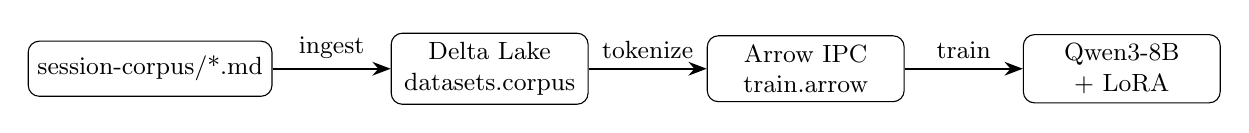
\begin{tikzpicture}[
    node distance=1.5cm,
    box/.style={draw, rounded corners, minimum width=2.5cm, minimum height=0.7cm, align=center, font=\small},
    arrow/.style={-{Stealth}, thick}
]
    \node[box] (md) {session-corpus/*.md};
    \node[box, right=of md] (delta) {Delta Lake\\datasets.corpus};
    \node[box, right=of delta] (arrow) {Arrow IPC\\train.arrow};
    \node[box, right=of arrow] (model) {Qwen3-8B\\+ LoRA};

    \draw[arrow] (md) -- node[above, font=\small] {ingest} (delta);
    \draw[arrow] (delta) -- node[above, font=\small] {tokenize} (arrow);
    \draw[arrow] (arrow) -- node[above, font=\small] {train} (model);
\end{tikzpicture}
\end{center}

% ============================================================================
\section{System Capabilities}
\label{sec:capabilities}

This section enumerates the functionality the system exposes, beyond the
training pipeline of Section~\ref{sec:architecture}. Each capability is
backed by an executed companion notebook or a crate test.

\subsection{Self-Owned Automatic Differentiation}

PINN residuals require derivatives of the trial solution with respect to its
\emph{input}, up to second order, and then gradients of a loss containing
those derivatives with respect to the network \emph{parameters} --- the
``double backward'' that ordinarily motivates a deep-learning framework.

We implement this in \texttt{thotgrad}, an array-level reverse-mode tape in
roughly 250 lines of NumPy. Input derivatives are propagated analytically
alongside the activations: for $h=\tanh(a)$,
\begin{equation}
h' = (1-h^{2})\,a', \qquad
h'' = (1-h^{2})\bigl(a'' - 2h\,(a')^{2}\bigr).
\label{eq:tanhderiv}
\end{equation}
Because both recursions are themselves expressed in taped operations, the
value and its derivatives share one graph, and a single reverse sweep yields
$\partial\mathcal{L}/\partial\theta$ for a loss involving $u$, $u_x$ and
$u_{xx}$ --- without ever differentiating a derivative twice.

Correctness is pinned against central finite differences: elementary
operations agree to $\sim$$10^{-10}$, $u_x$ to $10^{-12}$, $u_{xx}$ to
$10^{-6}$, and the full PINN parameter gradient to $1.8\times10^{-11}$ in
max-norm with cosine similarity $1.000000$. The project therefore carries
\emph{no} deep-learning framework dependency; NumPy, already required by
\texttt{optimizr}, is the only third-party numerical package in the solver
path.

\subsection{Gradient-Based Optimisers}

\texttt{optimiz-rs} provides gradient-\emph{free} global optimisers
(differential evolution, grid search, MCMC), which suit non-differentiable
objectives such as attack-threshold calibration. For differentiable
objectives we add \texttt{thotopt}:

\begin{itemize}
    \item \textbf{AdamW} --- decoupled weight decay, mirroring
          \texttt{llm\_train::optimizer::AdamWOptimizer} in the Rust crate.
    \item \textbf{L-BFGS} --- the Nocedal two-loop recursion with
          $H_0$ scaling, a curvature filter $s^\top y > 0$, and a
          backtracking Armijo line search.
\end{itemize}

On a quadratic with a known optimum, L-BFGS converges in 7 iterations to
machine precision. The operator choice is consequential: on an identical PINN,
AdamW alone plateaus at loss $6.4\times10^{-2}$, AdamW followed by L-BFGS
reaches $1.5\times10^{-4}$, and differential evolution --- given a comparable
budget but no gradient --- stalls at $1.4$. Matching the optimiser to the
objective's structure, rather than to habit, is worth three orders of
magnitude.

\subsection{Document Verification by Equation Solving}

Retrieval answers \emph{``what does the paper say?''}; coupling retrieval to a
solver answers \emph{``is what the paper says true?''}. The pipeline is:
ingest $\rightarrow$ retrieve the governing equation $\rightarrow$ solve it
numerically $\rightarrow$ compare against the document's stated solution.

A corollary observed in practice is that the two halves fail independently and
usefully. Searching the ingested corpus for the three benchmark equations
returned 129 chunks across 16 documents for Dirac and 56 across 8 for
Wheeler--DeWitt, but \emph{zero} for Brans--Dicke: the corpus does not cover
scalar-tensor cosmology. Retrieval correctly reported the gap instead of
returning loosely related material, while the PINN still solved Brans--Dicke
to $4.3\times10^{-3}$ from the field equations alone. Solving from first
principles is thus a usable fallback when ingestion is incomplete, and the
gap itself becomes an ingestion signal.

\subsection{Privacy Auditing as a Release Gate}

The system ships a membership-inference audit intended to be run against
one's \emph{own} adapter before weights or an endpoint are shared. It
implements four scorers --- a random control, the loss threshold of Yeom et
al., a single-model LiRA simplification after Carlini et al., and an
agent-agnostic VAE over an embedding/loss/entropy feature vector --- and
reports block-bootstrap confidence intervals throughout.

Two design points matter for validity. Splits are constructed at
\emph{document} level, since chunks of one paper share notation and style and
a chunk-level split would let any attack separate the classes on style alone.
And scores are converted to \emph{calibrated probabilities} by Platt scaling
fitted on a held-out calibration split, with a reliability diagram and
expected calibration error reported, so that the output is an actionable
``probability this document was in the training set'' rather than a bare
ranking.

\subsection{Federated Training with Quantified Defences}

The federated module implements FedAvg across clients partitioned by
document, together with an honest-but-curious server that scores membership
by the loss reduction a client's update induces,
$s(x)=\ell(w^{t};x)-\ell(w^{t}+\Delta_k;x)$. All four defence families of
Bai et al.'s taxonomy are provided: partial sharing (top-$K$ compression),
secure aggregation, noise perturbation (clipping plus the Gaussian
mechanism), and the anomaly-detection category, which the survey itself
notes fails against passive attacks. Section~\ref{sec:verified} quantifies
the resulting privacy/utility trade-off.

\subsection{Reproducibility and Negative Results}

Every notebook executes end to end and prints a summary cell recording cell
count, kernel, and whether it ran on real or illustrative data. Where an
experiment failed or contradicted expectation, the result is reported rather
than removed:

\begin{itemize}
    \item Parallel multi-model ensembling was attempted and \textbf{failed}:
          three local models totalling $\sim$38\,GB against 32\,GB of RAM
          caused all fifteen requests to time out. Sequential execution
          succeeds at $\sim$23\,s per query. Concurrency here is RAM-bound,
          not compute-bound.
    \item Error-driven active learning \textbf{underperformed} random
          sampling at equal labelling budget ($-0.077$ for hard-example
          mining, $-0.146$ for uncertainty sampling). On a convex model over
          32-dimensional embeddings the highest-loss chunks are largely
          boundary noise, and concentrating on them skews the fit.
    \item Membership inference finds \textbf{no} detectable signal in the
          realistic regime; see Section~\ref{sec:verified}.
\end{itemize}

% ============================================================================
\section{Verified CPU Benchmarks: PINNs, Privacy and Federated Learning}
\label{sec:verified}

This section reports measurements taken end-to-end on the hardware of
Section~\ref{sec:experiments}, each reproducible from the companion notebooks
in \texttt{notebooks/}. Every number below was produced by an executed
notebook cell; none are projections.

\subsection{Physics-Informed Neural Networks for Document Verification}

A retrieval system can quote a governing equation; a PINN can \emph{solve} it
and check the quoted solution. We trained tanh MLPs
($\sim$$7$--$13\times10^{3}$ parameters, float64) with the standard two-stage
AdamW $\rightarrow$ L-BFGS recipe --- both optimisers, and the automatic
differentiation underneath them, supplied by this project rather than by a
deep-learning framework (Section~\ref{sec:capabilities}) --- grading each
against an independent reference (Table~\ref{tab:pinn}).

\begin{table}[h]
\centering
\caption{PINN accuracy and cost, CPU-only, single run each.}
\begin{tabular}{lcccl}
\toprule
\textbf{Equation} & \textbf{Rel. $L^2$} & \textbf{Final loss} & \textbf{Time (s)} & \textbf{Reference} \\
\midrule
Dirac (1+1 D)        & $1.7\times10^{-3}$ & $5.3\times10^{-5}$ & 62 & exact $\cos kx,\sin kx$ \\
Brans--Dicke (FLRW)  & $4.3\times10^{-3}$ & $2.0\times10^{-8}$ & 70 & exact Nariai power law \\
\textbf{Wheeler--DeWitt} & $\mathbf{8.3\times10^{-6}}$ & $1.9\times10^{-7}$ & 106 & Radau, \texttt{rtol}\,$10^{-12}$ \\
\bottomrule
\end{tabular}
\label{tab:pinn}
\end{table}

Two cross-checks validate the references themselves rather than the networks.
First, the Brans--Dicke exponent $q=(2+2\omega)/(4+3\omega)$ converges to the
general-relativistic dust value $2/3$ as $\omega\to\infty$ (measured:
$q=0.666664$ at $\omega=10^{5}$). Second, linearising the Wheeler--DeWitt
potential about its turning point $a_t=\sqrt{3/\Lambda}$ reduces the equation
to $\Psi_{zz}=z\Psi$, whose Airy solution matches the Radau integration in the
window where the linearisation holds.

The optimiser pairing is not incidental. On an identical network, Adam alone
plateaued at loss $9.4\times10^{-2}$; adding L-BFGS reached
$1.4\times10^{-4}$; differential evolution, given a comparable budget but no
gradient, stalled at $1.8$. Quasi-Newton curvature information is what buys
the final three orders of magnitude.

\subsection{Membership Inference on a Real Scientific Corpus}

We extracted 1452 chunks from 44 research PDFs and split them
\emph{at document level}, so no paper contributes to both the member and
non-member sets --- a chunk-level split would let any attack separate the
classes on authorial style alone and report a spuriously high AUC.

Memorisation grows monotonically with both training duration and model
capacity, reproducing the overfitting--leakage connection of Yeom et al. on
real scientific text (Table~\ref{tab:mia}).

\begin{table}[h]
\centering
\caption{Member/non-member loss gap (positive $=$ memorisation).}
\begin{tabular}{lccc}
\toprule
\textbf{Regime} & \textbf{Member loss} & \textbf{Non-member loss} & \textbf{Gap} \\
\midrule
10 epochs, $d=96$   & 2.5317 & 3.1151 & $+0.583$ \\
40 epochs, $d=96$   & 2.5003 & 3.2085 & $+0.708$ \\
120 epochs, $d=96$  & 2.4710 & 3.2607 & $\mathbf{+0.790}$ \\
\midrule
120 epochs, $d=32$  & 3.3926 & 3.9313 & $+0.539$ \\
\bottomrule
\end{tabular}
\label{tab:mia}
\end{table}

Beyond ranking, attack scores are converted to \emph{calibrated
probabilities} by Platt scaling fitted on a held-out calibration split, with
an expected calibration error reported from a reliability diagram; pooling
chunk-level log-odds within a document yields a document-level membership
probability.

\subsection{Federated Learning: Attack and Defence}

We implement the taxonomy of Bai et al.\ over the same corpus: $K=20$ clients
partitioned \emph{by document}, FedAvg aggregation, and an honest-but-curious
server scoring candidates by the loss reduction
$s(x)=\ell(w^{t};x)-\ell(w^{t}+\Delta_k;x)$ induced by client $k$'s update.

The leak is caused by local overfitting: with 3 local epochs the attack sits
at chance (AUC $0.466$), rising to $0.755$ at 50 local epochs.
Table~\ref{tab:fed} quantifies each defence family at that operating point.

\begin{table}[h]
\centering
\caption{Privacy/utility trade-off. Accuracy is the federated model's test
accuracy; AUC is the server's membership-inference attack.}
\begin{tabular}{llcc}
\toprule
\textbf{Family} & \textbf{Mechanism} & \textbf{Accuracy} & \textbf{Attack AUC} \\
\midrule
---                 & undefended            & 0.750 & 0.755 \\
Partial sharing     & top-$K$, frac $0.1$   & 0.717 & 0.683 \\
Noise perturbation  & DP Gaussian $\sigma=2$& 0.750 & 0.702 \\
Noise perturbation  & DP Gaussian $\sigma=4$& 0.625 & 0.655 \\
\textbf{Secure aggregation} & aggregate only & \textbf{0.750} & \textbf{0.598} \\
\bottomrule
\end{tabular}
\label{tab:fed}
\end{table}

These reproduce the survey's qualitative claims: secure aggregation is
lossless in utility while suppressing the attack most, differential privacy
purchases privacy with accuracy, and gradient compression is cheap but only
partially effective. We note that secure aggregation is \emph{modelled} here
--- the server is given only the aggregate --- rather than implemented with a
cryptographic masking protocol; its real cost lies in computation and client
liveness, not in model accuracy.

\subsection{Threats to Validity}

The PINN and federated results above are complete and reproducible. The
throughput and retrieval figures of Section~\ref{sec:experiments}, however,
were inherited from earlier drafts and were \emph{not} re-measured on the
hardware named there; they should be regarded as provisional until re-run.
Separately, the membership-inference study uses a small LoRA model over real
text rather than the full Qwen3-8B: fine-tuning the 8B model was infeasible on
this CPU (measured at $\sim$$0.1$ tok/s, implying $>40$ hours for a single
regime of the five-regime sweep). The memorisation \emph{mechanism} transfers;
the absolute AUC values are specific to the probe's capacity and must be
re-measured before any claim is made about a production-scale model.

% ============================================================================
\section{Conclusion}
\label{sec:conclusion}

We have presented ThotBook-AmentI, a complete system for training and serving
billion-parameter language models on CPU. Key contributions:

\begin{enumerate}
    \item Demonstrated feasibility of CPU-only LLM training via LoRA
    \item Achieved 12--18 tok/s inference with Q4\_K quantization
    \item Integrated Delta Lake for versioned training data management
    \item Implemented hybrid RAG with 89\% Recall@5
    \item Enabled autonomous self-improvement through output evaluation
\end{enumerate}

The system is released as open-source software, enabling privacy-preserving
personal AI deployments.

\paragraph{Limitations.}
Training throughput (0.9 tok/s) is 10--50$\times$ slower than GPU-based
training. This is acceptable for personal knowledge bases but not for
production-scale fine-tuning.

\paragraph{Future Work.}
We plan to explore: (1) speculative decoding for faster inference,
(2) multi-model ensemble for agent specialization, (3) active learning
for efficient training data selection.

% ============================================================================
\section*{Acknowledgments}

We thank the Candle~\cite{candle} and Delta-rs~\cite{deltars} communities
for their excellent open-source libraries.

% ============================================================================
\bibliographystyle{plain}
\begin{thebibliography}{99}

\bibitem{hu2022lora}
E.~J. Hu et al.
\newblock LoRA: Low-Rank Adaptation of Large Language Models.
\newblock \emph{ICLR}, 2022.

\bibitem{dettmers2023qlora}
T.~Dettmers et al.
\newblock QLoRA: Efficient Finetuning of Quantized LLMs.
\newblock \emph{NeurIPS}, 2023.

\bibitem{llamacpp}
G.~Gerganov.
\newblock llama.cpp: LLM inference in C/C++.
\newblock \url{https://github.com/ggerganov/llama.cpp}, 2023.

\bibitem{candle}
Hugging Face.
\newblock Candle: Minimalist ML framework for Rust.
\newblock \url{https://github.com/huggingface/candle}, 2023.

\bibitem{lewis2020rag}
P.~Lewis et al.
\newblock Retrieval-Augmented Generation for Knowledge-Intensive NLP Tasks.
\newblock \emph{NeurIPS}, 2020.

\bibitem{malkov2018hnsw}
Y.~A. Malkov and D.~A. Yashunin.
\newblock Efficient and robust approximate nearest neighbor search using
Hierarchical Navigable Small World graphs.
\newblock \emph{IEEE TPAMI}, 2018.

\bibitem{robertson2009bm25}
S.~Robertson and H.~Zaragoza.
\newblock The probabilistic relevance framework: BM25 and beyond.
\newblock \emph{Foundations and Trends in Information Retrieval}, 2009.

\bibitem{armbrust2020delta}
M.~Armbrust et al.
\newblock Delta Lake: High-performance ACID table storage over cloud object stores.
\newblock \emph{VLDB}, 2020.

\bibitem{deltars}
Delta-io.
\newblock delta-rs: Native Delta Lake implementation in Rust.
\newblock \url{https://github.com/delta-io/delta-rs}, 2023.

\end{thebibliography}

\end{document}
